\documentclass{book}
\usepackage[a4paper,top=2.5cm,bottom=2.5cm,left=2.5cm,right=2.5cm]{geometry}
\usepackage{makeidx}
\usepackage{natbib}
\usepackage{graphicx}
\usepackage{multicol}
\usepackage{float}
\usepackage{listings}
\usepackage{color}
\usepackage{ifthen}
\usepackage[table]{xcolor}
\usepackage{textcomp}
\usepackage{alltt}
\usepackage{ifpdf}
\ifpdf
\usepackage[pdftex,
            pagebackref=true,
            colorlinks=true,
            linkcolor=blue,
            unicode
           ]{hyperref}
\else
\usepackage[ps2pdf,
            pagebackref=true,
            colorlinks=true,
            linkcolor=blue,
            unicode
           ]{hyperref}
\usepackage{pspicture}
\fi
\usepackage[utf8]{inputenc}
\usepackage{polski}
\usepackage[T1]{fontenc}

\usepackage{mathptmx}
\usepackage[scaled=.90]{helvet}
\usepackage{courier}
\usepackage{sectsty}
\usepackage{amssymb}
\usepackage[titles]{tocloft}
\usepackage{doxygen}
\lstset{language=C++,inputencoding=utf8,basicstyle=\footnotesize,breaklines=true,breakatwhitespace=true,tabsize=4,numbers=left }
\makeindex
\setcounter{tocdepth}{3}
\renewcommand{\footrulewidth}{0.4pt}
\renewcommand{\familydefault}{\sfdefault}
\hfuzz=15pt
\setlength{\emergencystretch}{15pt}
\hbadness=750
\tolerance=750
\begin{document}
\hypersetup{pageanchor=false,citecolor=blue}
\begin{titlepage}
\vspace*{7cm}
\begin{center}
{\Large My Project }\\
\vspace*{1cm}
{\large Wygenerowano przez Doxygen 1.8.3.1}\\
\vspace*{0.5cm}
{\small So, 24 maj 2014 22:18:33}\\
\end{center}
\end{titlepage}
\clearemptydoublepage
\pagenumbering{roman}
\tableofcontents
\clearemptydoublepage
\pagenumbering{arabic}
\hypersetup{pageanchor=true,citecolor=blue}
\chapter{Dokumentacja zadania lab9}
\label{index}\hypertarget{index}{}\begin{DoxyAuthor}{Autor}
Karolina Morawska 
\end{DoxyAuthor}
\begin{DoxyDate}{Data}
16.\-03.\-2014 
\end{DoxyDate}
\begin{DoxyVersion}{Wersja}
0.\-2 
\end{DoxyVersion}

\chapter{Indeks klas}
\section{Lista klas}
Tutaj znajdują się klasy, struktury, unie i interfejsy wraz z ich krótkimi opisami\-:\begin{DoxyCompactList}
\item\contentsline{section}{\hyperlink{class_n_o_d_e}{N\-O\-D\-E} \\*Modeluje pojęcie \hyperlink{class_n_o_d_e}{N\-O\-D\-E} ,czyli wezel. Klasa modeluje pojęcie node . Jej atrybutem są pola zawierające wskaźnik na lewy ,prawy węzeł i wartość }{\pageref{class_n_o_d_e}}{}
\item\contentsline{section}{\hyperlink{class_para}{Para} \\*Modeluje pojęcie \hyperlink{class_para}{Para}. Klasa modeluje pojęcie para . Jej atrybutem są pola zawierające klucz i wartość }{\pageref{class_para}}{}
\item\contentsline{section}{\hyperlink{classper}{per$<$ K, W $>$} \\*Modeluje pojęcie per. Klasa modeluje pojęcie per(para) . Jej atrybutem są pola zawierające klucz i wartość }{\pageref{classper}}{}
\item\contentsline{section}{\hyperlink{class_tablicaas}{Tablicaas$<$ K, W $>$} \\*Modeluje pojęcie \hyperlink{class_tablicaas}{Tablicaas}. Klasa modeluje pojęcie Tablica asocjacyjna . Jej atrybutem są pola zawierające klucz i wartość }{\pageref{class_tablicaas}}{}
\item\contentsline{section}{\hyperlink{class_tree}{Tree} \\*Modeluje pojęcie \hyperlink{class_para}{Para}. Klasa modeluje pojęcie para . Jej atrybutem jest pole zawierajace root(korzen) }{\pageref{class_tree}}{}
\end{DoxyCompactList}

\chapter{Indeks plików}
\section{Lista plików}
Tutaj znajduje się lista wszystkich plików z ich krótkimi opisami\-:\begin{DoxyCompactList}
\item\contentsline{section}{\hyperlink{czas_8hh}{czas.\-hh} }{\pageref{czas_8hh}}{}
\item\contentsline{section}{\hyperlink{dzialania_8cpp}{dzialania.\-cpp} }{\pageref{dzialania_8cpp}}{}
\item\contentsline{section}{\hyperlink{dzialania_8hh}{dzialania.\-hh} }{\pageref{dzialania_8hh}}{}
\item\contentsline{section}{\hyperlink{kolejka_8hh}{kolejka.\-hh} }{\pageref{kolejka_8hh}}{}
\item\contentsline{section}{\hyperlink{main_8cpp}{main.\-cpp} }{\pageref{main_8cpp}}{}
\item\contentsline{section}{\hyperlink{stos_8hh}{stos.\-hh} }{\pageref{stos_8hh}}{}
\item\contentsline{section}{\hyperlink{stos2_8hh}{stos2.\-hh} }{\pageref{stos2_8hh}}{}
\item\contentsline{section}{\hyperlink{stoslista_8hh}{stoslista.\-hh} }{\pageref{stoslista_8hh}}{}
\item\contentsline{section}{\hyperlink{tablica_8cpp}{tablica.\-cpp} }{\pageref{tablica_8cpp}}{}
\item\contentsline{section}{\hyperlink{tablica_8hh}{tablica.\-hh} }{\pageref{tablica_8hh}}{}
\end{DoxyCompactList}

\chapter{Dokumentacja klas}
\hypertarget{classplecak}{\section{Dokumentacja klasy plecak}
\label{classplecak}\index{plecak@{plecak}}
}


Modeluje pojęcie plecak. Jej atrybutem jest wektor ktory zawiera elementy dodawane do plecaka.  




{\ttfamily \#include $<$plecak.\-h$>$}

\subsection*{Metody publiczne}
\begin{DoxyCompactItemize}
\item 
void \hyperlink{classplecak_a03475949d5e5613bdeaa2311465fac93}{oblicz} (vector$<$ pair$<$ int, int $>$ $>$ \hyperlink{classplecak_aa4925fd62ae61e120cae3409d97a12bb}{T}, int maxpoj)
\begin{DoxyCompactList}\small\item\em Metoda glowna programu, oblicza jak najlepsze zapelnienie plecaka. Jej atrybutami są wektor T i max pojemnosc plecaka. \end{DoxyCompactList}\item 
int \hyperlink{classplecak_ac71a254ad6907aaf40fe17d845dda799}{wartosc} (int poj)
\begin{DoxyCompactList}\small\item\em Metoda sluzy do zwracania wartosci przedmiotu. \end{DoxyCompactList}\item 
vector$<$ pair$<$ int, int $>$ $>$ \hyperlink{classplecak_a54c09cbd49dc74a905686731575c2fe5}{przedmioty} (int poj)
\begin{DoxyCompactList}\small\item\em Pomocniczy metoda zwracajaca elementy ktorymi zostal zapelniony plecak. \end{DoxyCompactList}\item 
\hyperlink{classplecak_ae4a83a03f80233a82ca1d2d1f963432a}{plecak} ()
\begin{DoxyCompactList}\small\item\em Inicjalizuje konstruktor. \end{DoxyCompactList}\item 
virtual \hyperlink{classplecak_a918a266d6f8e95439b6ba37c1f6b41cf}{$\sim$plecak} ()
\begin{DoxyCompactList}\small\item\em Inicjalizuje wirtualny konstruktor. \end{DoxyCompactList}\end{DoxyCompactItemize}
\subsection*{Atrybuty publiczne}
\begin{DoxyCompactItemize}
\item 
vector$<$ pair$<$ int, int $>$ $>$ \hyperlink{classplecak_aa4925fd62ae61e120cae3409d97a12bb}{T}
\begin{DoxyCompactList}\small\item\em Zmienna wektor ktora przechowuje pare\-: waga i wartosc elementu. \end{DoxyCompactList}\item 
vector$<$ int $>$ \hyperlink{classplecak_a42a413a1022b907eaf87605b17c86738}{maxvalue}
\begin{DoxyCompactList}\small\item\em Zmienna wektor ktora przechowuje maksymalna wartosc jaka mozna wlozyc do plecaka. \end{DoxyCompactList}\item 
vector$<$ int $>$ \hyperlink{classplecak_a347d5be822af6095956944e815df0473}{lastitem}
\begin{DoxyCompactList}\small\item\em Zmienna wektor, przechowuje ostatni dodany element. \end{DoxyCompactList}\end{DoxyCompactItemize}


\subsection{Opis szczegółowy}


Definicja w linii 25 pliku plecak.\-h.



\subsection{Dokumentacja konstruktora i destruktora}
\hypertarget{classplecak_ae4a83a03f80233a82ca1d2d1f963432a}{\index{plecak@{plecak}!plecak@{plecak}}
\index{plecak@{plecak}!plecak@{plecak}}
\subsubsection[{plecak}]{\setlength{\rightskip}{0pt plus 5cm}plecak\-::plecak (
\begin{DoxyParamCaption}
{}
\end{DoxyParamCaption}
)}}\label{classplecak_ae4a83a03f80233a82ca1d2d1f963432a}


Definicja w linii 13 pliku plecak.\-cpp.

\hypertarget{classplecak_a918a266d6f8e95439b6ba37c1f6b41cf}{\index{plecak@{plecak}!$\sim$plecak@{$\sim$plecak}}
\index{$\sim$plecak@{$\sim$plecak}!plecak@{plecak}}
\subsubsection[{$\sim$plecak}]{\setlength{\rightskip}{0pt plus 5cm}plecak\-::$\sim$plecak (
\begin{DoxyParamCaption}
{}
\end{DoxyParamCaption}
)\hspace{0.3cm}{\ttfamily [virtual]}}}\label{classplecak_a918a266d6f8e95439b6ba37c1f6b41cf}


Definicja w linii 18 pliku plecak.\-cpp.



\subsection{Dokumentacja funkcji składowych}
\hypertarget{classplecak_a03475949d5e5613bdeaa2311465fac93}{\index{plecak@{plecak}!oblicz@{oblicz}}
\index{oblicz@{oblicz}!plecak@{plecak}}
\subsubsection[{oblicz}]{\setlength{\rightskip}{0pt plus 5cm}void plecak\-::oblicz (
\begin{DoxyParamCaption}
\item[{vector$<$ pair$<$ int, int $>$ $>$}]{T, }
\item[{int}]{maxpoj}
\end{DoxyParamCaption}
)}}\label{classplecak_a03475949d5e5613bdeaa2311465fac93}


Definicja w linii 22 pliku plecak.\-cpp.



Oto graf wywoływań tej funkcji\-:\nopagebreak
\begin{figure}[H]
\begin{center}
\leavevmode
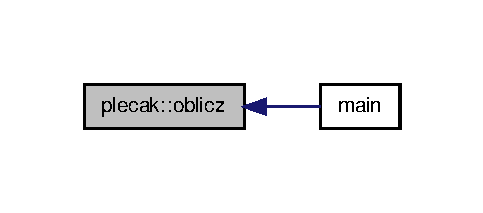
\includegraphics[width=232pt]{classplecak_a03475949d5e5613bdeaa2311465fac93_icgraph}
\end{center}
\end{figure}


\hypertarget{classplecak_a54c09cbd49dc74a905686731575c2fe5}{\index{plecak@{plecak}!przedmioty@{przedmioty}}
\index{przedmioty@{przedmioty}!plecak@{plecak}}
\subsubsection[{przedmioty}]{\setlength{\rightskip}{0pt plus 5cm}vector$<$ pair$<$ int, int $>$ $>$ plecak\-::przedmioty (
\begin{DoxyParamCaption}
\item[{int}]{poj}
\end{DoxyParamCaption}
)}}\label{classplecak_a54c09cbd49dc74a905686731575c2fe5}


Definicja w linii 47 pliku plecak.\-cpp.



Oto graf wywoływań tej funkcji\-:\nopagebreak
\begin{figure}[H]
\begin{center}
\leavevmode
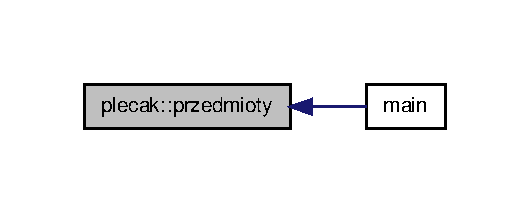
\includegraphics[width=254pt]{classplecak_a54c09cbd49dc74a905686731575c2fe5_icgraph}
\end{center}
\end{figure}


\hypertarget{classplecak_ac71a254ad6907aaf40fe17d845dda799}{\index{plecak@{plecak}!wartosc@{wartosc}}
\index{wartosc@{wartosc}!plecak@{plecak}}
\subsubsection[{wartosc}]{\setlength{\rightskip}{0pt plus 5cm}int plecak\-::wartosc (
\begin{DoxyParamCaption}
\item[{int}]{poj}
\end{DoxyParamCaption}
)}}\label{classplecak_ac71a254ad6907aaf40fe17d845dda799}


Definicja w linii 38 pliku plecak.\-cpp.



Oto graf wywoływań tej funkcji\-:\nopagebreak
\begin{figure}[H]
\begin{center}
\leavevmode
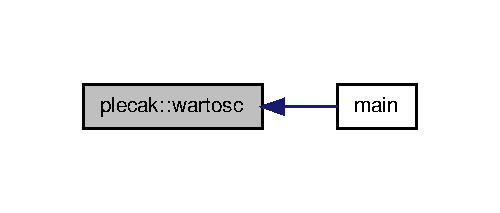
\includegraphics[width=240pt]{classplecak_ac71a254ad6907aaf40fe17d845dda799_icgraph}
\end{center}
\end{figure}




\subsection{Dokumentacja atrybutów składowych}
\hypertarget{classplecak_a347d5be822af6095956944e815df0473}{\index{plecak@{plecak}!lastitem@{lastitem}}
\index{lastitem@{lastitem}!plecak@{plecak}}
\subsubsection[{lastitem}]{\setlength{\rightskip}{0pt plus 5cm}vector$<$int$>$ plecak\-::lastitem}}\label{classplecak_a347d5be822af6095956944e815df0473}


Definicja w linii 39 pliku plecak.\-h.

\hypertarget{classplecak_a42a413a1022b907eaf87605b17c86738}{\index{plecak@{plecak}!maxvalue@{maxvalue}}
\index{maxvalue@{maxvalue}!plecak@{plecak}}
\subsubsection[{maxvalue}]{\setlength{\rightskip}{0pt plus 5cm}vector$<$int$>$ plecak\-::maxvalue}}\label{classplecak_a42a413a1022b907eaf87605b17c86738}


Definicja w linii 35 pliku plecak.\-h.

\hypertarget{classplecak_aa4925fd62ae61e120cae3409d97a12bb}{\index{plecak@{plecak}!T@{T}}
\index{T@{T}!plecak@{plecak}}
\subsubsection[{T}]{\setlength{\rightskip}{0pt plus 5cm}vector$<$pair$<$int,int$>$ $>$ plecak\-::\-T}}\label{classplecak_aa4925fd62ae61e120cae3409d97a12bb}


Definicja w linii 31 pliku plecak.\-h.



Dokumentacja dla tej klasy została wygenerowana z plików\-:\begin{DoxyCompactItemize}
\item 
/home/karolina/\-Pulpit/pamsi8/prj/\hyperlink{plecak_8h}{plecak.\-h}\item 
/home/karolina/\-Pulpit/pamsi8/prj/\hyperlink{plecak_8cpp}{plecak.\-cpp}\end{DoxyCompactItemize}

\chapter{Dokumentacja plików}
\hypertarget{main_8cpp}{\section{Dokumentacja pliku /home/karolina/\-Pulpit/pamsi/prj/src/main.cpp}
\label{main_8cpp}\index{/home/karolina/\-Pulpit/pamsi/prj/src/main.\-cpp@{/home/karolina/\-Pulpit/pamsi/prj/src/main.\-cpp}}
}
{\ttfamily \#include $<$iostream$>$}\\*
{\ttfamily \#include $<$dzialania.\-hh$>$}\\*
{\ttfamily \#include $<$cstdlib$>$}\\*
Wykres zależności załączania dla main.\-cpp\-:
\subsection*{Funkcje}
\begin{DoxyCompactItemize}
\item 
int \hyperlink{main_8cpp_a3c04138a5bfe5d72780bb7e82a18e627}{main} (int argc, char $\ast$$\ast$argv)
\begin{DoxyCompactList}\small\item\em Funkcja main wykonuje algorytm i sprawdza czas dzialania algorytmu. W funkcji main wykonywane sa operacje \-: -\/\-Wczytywanie pliku z danymi wejsciowym -\/\-Dane sa mnozone razy 2 (w tej chwili wlaczany jest stoper) -\/\-Wczytywanie pliku z danymi sprawdzajacymi -\/\-Sprawdzanie zgodnosci -\/\-Stoper zostaje wylaczony i na wyjsciu programu podany zostaje czas dzialania algorytmu. \end{DoxyCompactList}\end{DoxyCompactItemize}


\subsection{Dokumentacja funkcji}
\hypertarget{main_8cpp_a3c04138a5bfe5d72780bb7e82a18e627}{\index{main.\-cpp@{main.\-cpp}!main@{main}}
\index{main@{main}!main.cpp@{main.\-cpp}}
\subsubsection[{main}]{\setlength{\rightskip}{0pt plus 5cm}int main (
\begin{DoxyParamCaption}
\item[{int}]{argc, }
\item[{char $\ast$$\ast$}]{argv}
\end{DoxyParamCaption}
)}}\label{main_8cpp_a3c04138a5bfe5d72780bb7e82a18e627}


Funkcja main wykonuje algorytm i sprawdza czas dzialania algorytmu. W funkcji main wykonywane sa operacje \-: -\/\-Wczytywanie pliku z danymi wejsciowym -\/\-Dane sa mnozone razy 2 (w tej chwili wlaczany jest stoper) -\/\-Wczytywanie pliku z danymi sprawdzajacymi -\/\-Sprawdzanie zgodnosci -\/\-Stoper zostaje wylaczony i na wyjsciu programu podany zostaje czas dzialania algorytmu. 



Definicja w linii 22 pliku main.\-cpp.


\hypertarget{plecak_8cpp}{\section{Dokumentacja pliku /home/karolina/\-Pulpit/pamsi8/prj/plecak.cpp}
\label{plecak_8cpp}\index{/home/karolina/\-Pulpit/pamsi8/prj/plecak.\-cpp@{/home/karolina/\-Pulpit/pamsi8/prj/plecak.\-cpp}}
}


Funkcje do klasy plecak.  


{\ttfamily \#include \char`\"{}plecak.\-h\char`\"{}}\\*
Wykres zależności załączania dla plecak.\-cpp\-:\nopagebreak
\begin{figure}[H]
\begin{center}
\leavevmode
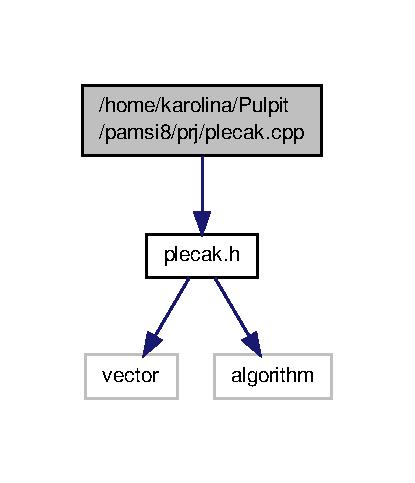
\includegraphics[width=199pt]{plecak_8cpp__incl}
\end{center}
\end{figure}

\hypertarget{plecak_8h}{\section{Dokumentacja pliku /home/karolina/\-Pulpit/pamsi8/prj/plecak.h}
\label{plecak_8h}\index{/home/karolina/\-Pulpit/pamsi8/prj/plecak.\-h@{/home/karolina/\-Pulpit/pamsi8/prj/plecak.\-h}}
}


Definicja klasy plecak.  


{\ttfamily \#include $<$vector$>$}\\*
{\ttfamily \#include $<$algorithm$>$}\\*
Wykres zależności załączania dla plecak.\-h\-:\nopagebreak
\begin{figure}[H]
\begin{center}
\leavevmode
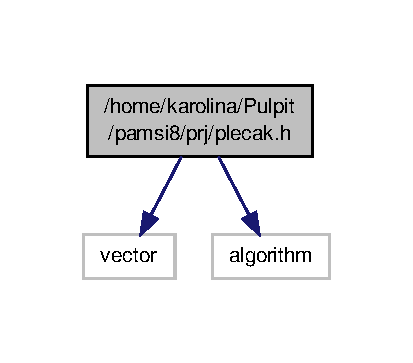
\includegraphics[width=198pt]{plecak_8h__incl}
\end{center}
\end{figure}
Ten wykres pokazuje, które pliki bezpośrednio lub pośrednio załączają ten plik\-:
\nopagebreak
\begin{figure}[H]
\begin{center}
\leavevmode
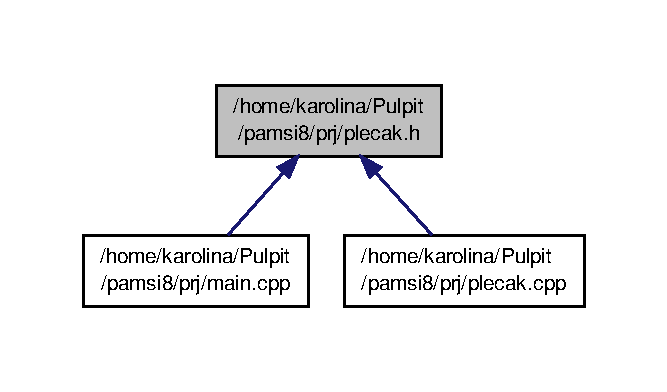
\includegraphics[width=320pt]{plecak_8h__dep__incl}
\end{center}
\end{figure}
\subsection*{Komponenty}
\begin{DoxyCompactItemize}
\item 
class \hyperlink{classplecak}{plecak}
\begin{DoxyCompactList}\small\item\em Modeluje pojęcie plecak. Jej atrybutem jest wektor ktory zawiera elementy dodawane do plecaka. \end{DoxyCompactList}\end{DoxyCompactItemize}


\subsection{Opis szczegółowy}
Plik zawiera definicję klasy Graf Jest to klasa glowna programu. 

Definicja w pliku \hyperlink{plecak_8h_source}{plecak.\-h}.


\addcontentsline{toc}{part}{Indeks}
\printindex
\end{document}
